\documentclass[titlepage, a4paper]{article}
\usepackage[english]{babel}
\usepackage[utf8]{inputenc}
\usepackage{graphicx}
\usepackage{color}
\usepackage{mathtools}
\usepackage{float}
\usepackage[parfill]{parskip}
\usepackage[margin=10pt,font=small,labelfont=bf,labelsep=endash]{caption}
\usepackage{epstopdf}
\usepackage{listings}
\epstopdfsetup{suffix=}
\DeclareGraphicsExtensions{.ps}
\DeclareGraphicsRule{.ps}{pdf}{.pdf}{`ps2pdf -dEPSCrop -dNOSAFER #1 \noexpand\OutputFile}

\lstset{literate=%
    {å}{{\r{a}}}1
    {ä}{{\"a}}1
    {ö}{{\"o}}1
    {Å}{{\r{A}}}1
    {Ä}{{\"A}}1
    {Ö}{{\"O}}1
}

\newcommand{\todo}[1] {\textbf{\textcolor{red}{#1}}}

\usepackage{fancyhdr}
\fancyhead[L]{}
\pagestyle{fancy}
\rhead{Alexander Yngve \\ Pål Kastman}
\chead{TDDC78}
\thispagestyle{empty}

\begin{document}

{\ }\vspace{45mm}

\begin{center}
  \Huge \textbf{TDDC78: Lab Report}
\end{center}
\begin{center}
  \Large Lab 1: MPI
\end{center}

\vspace{250pt}

\begin{center}
  \begin{tabular}{|*{3}{p{40mm}|}}
    \hline
    \textbf{Name} & \textbf{PIN} & \textbf{Email} \\ \hline
           {Alexander Yngve} & {930320-6651} & {aleyn573@student.liu.se} \\ \hline
           {Pål Kastman} & {851212-7575} & {palka285@student.liu.se} \\ \hline
  \end{tabular}
\end{center}
\newpage

\tableofcontents
\thispagestyle{empty}
\newpage

\section{Introduction}
This lab consists of two image filters: blur filter and threshold filter.

The goal of the lab is to distribute the workload to tasks running on different processes with the help of MPI. The tasks won't have access to the same data, so this needs to be sent.


\subsection{Blur filter}
The blur filter uses a normal distribution together with a given radius to calculate the mean value for every pixel in an image, this will create a blur the given image.


\subsection{Threshold filter}
The threshold filter first calculates a mean value for every pixel in the image, it will then go through the image one more time and either set every pixel to black or white depending if the pixel value is over or under the calculated mean value.

\section{Our implementation}
This section will describe how we used MPI to parallelize the execution of the programs.

It might be worth mentioning that we use MPI\_Barrier in both filters just for the sake of timing the filters, so that the timing starts and stops when all tasks are done with the filter.

\subsection{Blur filter}
For this filter we define an MPI type called mpi\_pixel\_type which contains a pixel, this will make it easier for us to send the data as we can send whole pixels instead of sending the r, b and g doubles of the pixel one by one.

We started by using MPI\_Send and MPI\_Recv to send parts of the image to the tasks. These parts were overlapping regions depending on how big the radius were, the size of them will also depend on how many tasks we have. This worked on our own laptops but unfortunately not on triolith for whatever reason we don't know. This made us instead use MPI\_Scatterv and MPI\_Gatherv as we had done for the threshold filter.

To be able to do this we must first broadcast the size in x and y, along with the radius, we do this with MPI\_Broadcast.

When the tasks have received their data, they will first run the blurfilter and then send the data back, without the overlapping regions.

After sending the data back, the tasks free their memory and runs MPI\_Finalize, which will kill them, except the first one which will save the result and free the memory before quiting.

\subsection{Threshold filter}
In this filter we also define the mpi\_pixel\_type just as for the blur filter. But because every pixel is just dependant on the actual value of the pixel, we won't need any overlap of the regions, and thus the MPI\_Scatterv and MPI\_Gatherv are instead used here.

We first broadcast the sizes in y and x along with the radius just as in the previous filter, then we send the regions to the different tasks and let them them calculate the average value of their areas. When all tasks are done with this, we run MPI\_Allgather which will make all tasks send their average value to all other tasks. So now all the tasks will calculate the average value independantly and then run the filter with this value.

When done, all tasks will send their data back to the first task and run MPI\_Finalize. The first task will save the result and free memory before quitting, just as in the previous filter.

\section{Execution times}
In this section we will present the execution times of the filters.

It is worth mentioning that the times for all graphs below are in seconds.

The tests were performed on four images with sizes as can be seen in \ref{tab:table1}.

\begin{table}[H]
  \centering
  \caption{The sizes for the images used in the tests.}
  \begin{tabular}{|*{3}{p{30mm}|}}
    \hline
    \textbf{Image name} & \textbf{x pixels } & \textbf{y pixels} \\ \hline
           {im1.ppm} & {676} & {763} \\ \hline
           {im2.ppm} & {1024} & {1024} \\ \hline
           {im3.ppm} & {1600} & {1200} \\ \hline
           {im4.ppm} & {3000} & {3000} \\ \hline
  \end{tabular}
  \label{tab:table1}
\end{table}

\subsection{Blur filter}
Here we saw that with an increase in the number of threads we get a decrease in time, which we wanted to attain.

Our result show that if we increase the number of threads, we will get a decrease in time. But this relationship is not linear due to deminishing returns, since the problem is not perfectly parallell the serial section sections start to dominate the execution time.

The results for image 1 and image 2 can the seen in figure \ref{fig:im1-blur} and figure \ref{fig:im2-blur} respectively. 


\begin{figure}[H]
  \centering
  \scalebox{0.48}{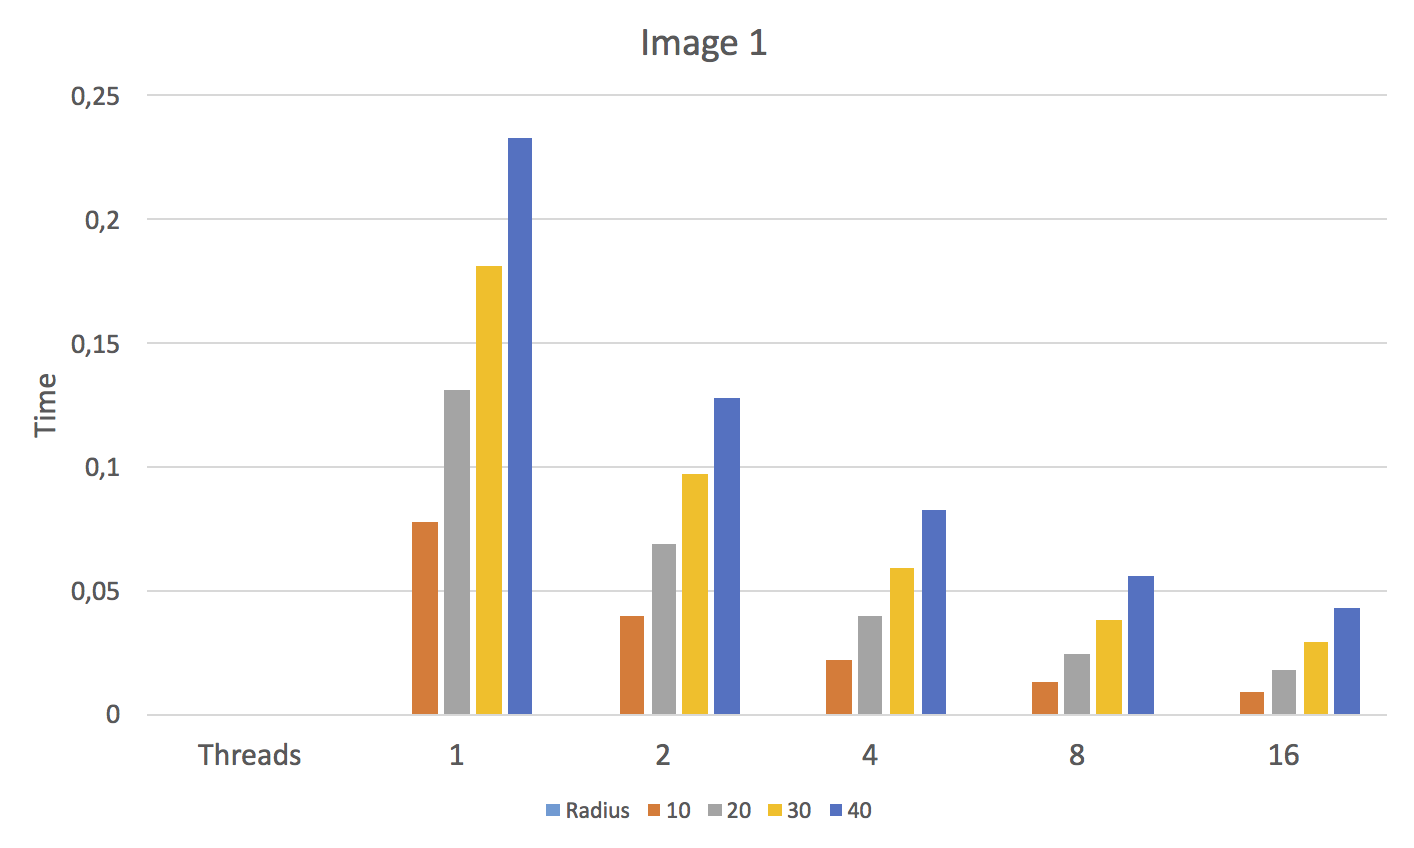
\includegraphics{img/im1-blur.png}}
  \caption{Result for the blurfilter run on image 1.}
  \label{fig:im1-blur}
\end{figure}

\begin{figure}[H]
  \centering
  \scalebox{0.48}{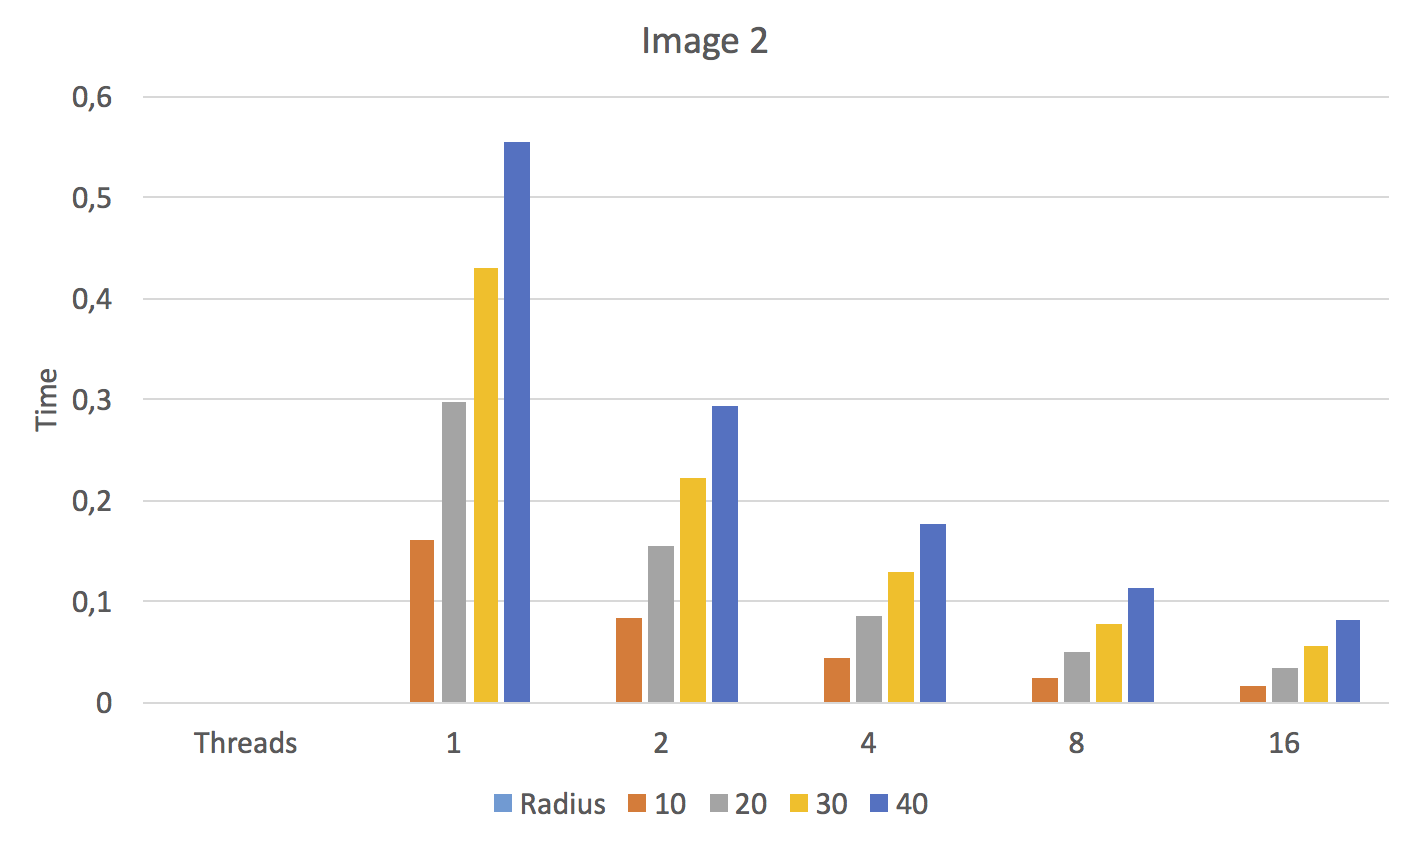
\includegraphics{img/im2-blur.png}}
  \caption{Result for the blurfilter run on image 2.}
  \label{fig:im2-blur}
\end{figure}


\subsection{Threshold filter}

\begin{figure}[H]
  \centering
  \scalebox{0.48}{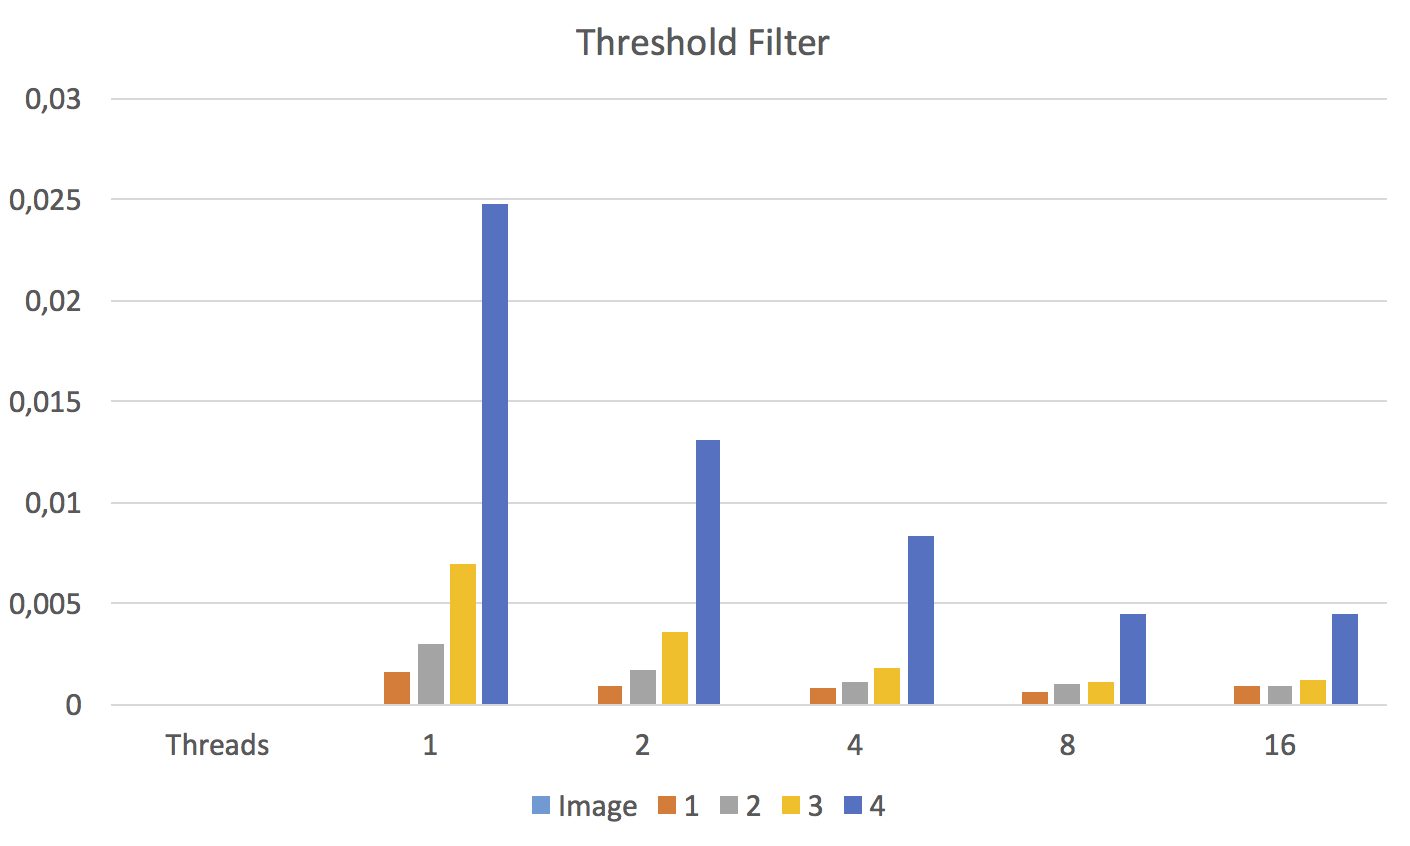
\includegraphics{img/threshold.png}}
  \caption{Result for the thresholdfilter.}
  \label{fig:threshold}
\end{figure}


\end{document}

%% \begin{table}[H]
%%   \centering
%%   \caption{Miss rates}
%%   \begin{tabular}{|*{3}{p{20mm}|}}
%%     \hline
%%     \textbf{Miss rates} & {test1} & {test2} \\ \hline
%%            {cache1} & {0.0091} & {0.1577} \\ \hline
%%            {cache2} & {0.0177} & {0.0235} \\ \hline
%%   \end{tabular}
%%   \label{tab:table1}
%% \end{table}


%% \begin{figure}[H]
%% 	\centering
%% 	\scalebox{0.342}{\includegraphics{img/data-cache.png}}
%% 	\caption{Only data stored in cache.}
%% 	\label{fig:data-cache}
%% \end{figure}
